\documentclass[12pt]{article}

\usepackage{graphicx}
\usepackage{amsmath}
\usepackage[margin=1in]{geometry}
\usepackage{fancyhdr}
\usepackage{enumerate}
\usepackage[shortlabels]{enumitem}
\usepackage[spanish]{babel}
\usepackage{xurl}
\usepackage{tcolorbox}
\usepackage{titlesec}
\usepackage{listings}
\usepackage{xcolor}
\usepackage{pgfplots}
\usepackage{tikz}

\titleclass{\subsubsubsection}{straight}[\subsection]

\newcounter{subsubsubsection}[subsubsection]
\renewcommand\thesubsubsubsection{\thesubsubsection.\arabic{subsubsubsection}}
\renewcommand\theparagraph{\thesubsubsubsection.\arabic{paragraph}} % optional; useful if paragraphs are to be numbered

\titleformat{\subsubsubsection}
{\normalfont\normalsize\bfseries}{\thesubsubsubsection}{1em}{}
\titlespacing*{\subsubsubsection}
{0pt}{3.25ex plus 1ex minus .2ex}{1.5ex plus .2ex}

\makeatletter
\renewcommand\paragraph{\@startsection{paragraph}{5}{\z@}%
  {3.25ex \@plus1ex \@minus.2ex}%
  {-1em}%
  {\normalfont\normalsize\bfseries}}
\renewcommand\subparagraph{\@startsection{subparagraph}{6}{\parindent}%
  {3.25ex \@plus1ex \@minus .2ex}%
  {-1em}%
  {\normalfont\normalsize\bfseries}}
\def\toclevel@subsubsubsection{4}
\def\toclevel@paragraph{5}
% \def\toclevel@paragraph{6}
\def\toclevel@subparagraph{6}
\def\l@subsubsubsection{\@dottedtocline{4}{7em}{4em}}
\def\l@paragraph{\@dottedtocline{5}{10em}{5em}}
\def\l@subparagraph{\@dottedtocline{6}{14em}{6em}}
\makeatother

\setcounter{secnumdepth}{4}
\setcounter{tocdepth}{4}

% Set up headers and footers
\pagestyle{fancy}
\fancyhf{}  % Clear previous settings

\fancyhead[L]{Alvarado Ludwig - Vera Julián}
\fancyhead[C]{Simulación Estocástica}
\fancyhead[R]{9 de Marzo de 2025}

\fancyfoot[C]{\thepage}
\fancyfoot[C]{\footnotesize Este trabajo está bajo una licencia CC 4.0. Más info: \url{https://creativecommons.org/licenses/by/4.0/}}

\renewcommand{\headrulewidth}{0.2pt}


% Define R Style for listings
\lstdefinestyle{RStyle}{
  language=R,
  basicstyle=\ttfamily\small,
  keywordstyle=\color{blue}\bfseries,
  commentstyle=\color{green!40!black}\itshape,
  stringstyle=\color{red!70!black},
  numbers=left,
  numberstyle=\tiny\color{gray},
  stepnumber=1,
  numbersep=5pt,
  backgroundcolor=\color{gray!10},
  showstringspaces=false,
  breaklines=true,
  frame=single,
  rulecolor=\color{black},
  captionpos=b,
  morekeywords={generator}
}

% Set RStyle as default
\lstset{style=RStyle}

\begin{document}

\tableofcontents


\section{\textit{Events and probability}}
\subsection{Punto a}
\subsubsection{Solución}

Se considera una caja con tres canicas de colores rojo, verde y ayuzal como la de la figura \ref{fig:caja-canica}, nos dicen que en el experimento se toma una canica y despues se vuelve a poner en la caja, es decir, si definimos los eventos como:

\begin{itemize}
  \item \(A\) sacar canica verde.
  \item \(B\) sacar canica azul.
  \item \(C\) sacar canica roja.
\end{itemize}

Se afirma que los eventos \(A, B\) y \(C\) son independientes los unos de los otros, ya que, estos no dependen del otro.

\begin{itemize}
  \item \textbf{Espacio muestral (\(\Omega\)):} de acuerdo a la definición ``Es el conjunto de todos los posibles resultados de un experimento aleatorio.'' En este experimento solo se pueden tener diferentes pares de resultados Por lo tanto, la combinación de estos resultados da como resultado el siguiente conjunto:
        \[
        \Omega = \{ (A,A), (A, B), (A, C), (B, A), (B, B), (B, C), (C, A), (C, B), (C, C)  \}
        \]
        Al sacar \(|\Omega|\) este resultado es de \(9\) posibles resultados del experimento. 
  \item \textbf{Probabilidad de cada canica:} el enunciado nos dice que cada canica tiene el mismo chance de ser seleccionada, es decir, una entre tres canicas, por lo tanto, las probabilidades de cada evento se definen como:
        \[
        P(A) = \frac{1}{3} = 0.33\overline{333} \qquad P(B) = \frac{1}{3} = 0.33\overline{333} \qquad P(C) = \frac{1}{3} = 0.33\overline{333}
        \]
        Las dos sacadas son independientes, por lo tanto, se puede aplicar que para cada par \((X, Y)\) se cumpla:
        \[
        P(X) \times P(Y) = \frac{1}{3} \times \frac{1}{3} = \frac{1}{9} = 0.11\overline{111}
        \]
        Por lo tanto, cada punto en el espacio muestral es de \(\frac{1}{9}\).
\end{itemize}



\begin{figure}[ht]
  \centering
  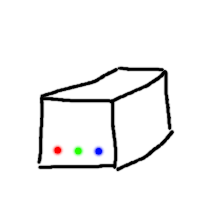
\includegraphics[width=0.4\textwidth]{img/Caja.png}
  \caption{\label{fig:caja-canica} Caja con 3 canicas de colores rojo, verde y azul. Ilustración de los autores elaborada en el software GIMP.}
\end{figure}


\subsection{Punto b}
\subsubsection{Solución}

En este punto nos plantean la misma situación anterior pero los eventos son \textbf{dependientes}, ya que, se saca la primera canica y no se vuelve a meter, es decir, si saco la canica azul como se ve en la figura \ref{fig:caja-2} para la segunda sacada de canica la probabilidad no va a ser la misma, puesto que, hay únicamente dos canicas a sacar. 

\begin{figure}[ht]
  \centering
  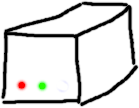
\includegraphics[width=.3\textwidth]{img/Caja2.png}
  \caption{\label{fig:caja-2} Caja con canicas verde y roja. Ilustración de los autores elaborada en el software GIMP.}
\end{figure}


Entonces, el conjunto del espacio muestral \(\Omega\) queda como:

\[
  \Omega = \{ (A, B), (A, C), (B, A), (B, C), (C, A), (C, B)\}
\]

La cardinalidad entonces del conjunto \(\Omega\) es de 6.

Teniendo en cuenta la probabilidad para dos eventos dependientes:

\[
  P(X \cap Y) = P(X|Y) P(Y)
\]

Si sacamos una canica de color rojo (\(P(C)\)) su probabilidad se mantiene como la del mundo anterior \(\frac{1}{3}\). Podemos deducir que en el espacio muestral quedan las canicas azul y verde, si deseamos sacar la azul \((P(B)\), esta está condicionada por el evento anterior de sacar la roja. Teniendo en cuenta, lo anterior, la probabilidad de sacar una canica azul será \(P(B|C) = \frac{1}{2}\). Por lo tanto, al realizar la operación:

\[
  P(B|C)P(C) = \frac{1}{2} \times \frac{1}{3} = \frac{1}{6} = 0.166\overline{666}
\]

Generalizando con \((X, Y)\) siendo un par del espacio muestral \(\Omega\):

\[
  P(X \cap Y) = P(X|Y)P(Y) = \frac{1}{2} \times \frac{1}{3} = \frac{1}{6} =  0.166\overline{666}
\]

En conclusión, la probabilidad para cada canica dado que se saque una antes y no se vuelva a introducir es de \(0.166\overline{666}\). 

\section{\textit{Congruential generators}}
\subsection{Solución}

La solución a este ejercicio se puede ver a más profundidad en el archivo \textsf{R} \textit{markdown} adjunto.  

Teniendo en cuenta el siguiente generador:

\[
  X_{n} = (9X_{n-1} + 3) \mod 11
\]

Se utiliza la siguiente función \lstinline|generator()| programada en \textsf{R}.

\begin{lstlisting}
generator <- function(x_n1, n){
  for (i in 1:n){
    print(x_n1)
    x_n1 <- (9 * x_n1 + 3) %% 11
  }
}
\end{lstlisting}

Los \textit{seeds} o semillas ($X_{n-1}$) que sirven para generar todos los ciclos son:

\begin{itemize}
  \item $X_{n-1} = 1:$ Se obtiene la siguiente secuencia $\{1, 1, \cdots \}$, un conjunto de solo unos.
  \item $X_{n-1} = 2:$ Se obtiene $\{2, 10, 5, 4, 6, 2, 10, \cdots \}$.
  \item $X_{n-1} = 3:$ El conjunto es $\{3, 8, 9, 7, 0, 3, 8, \cdots \} $.
\end{itemize}

Al llamar las funciones con estas semillas, se obtiene:

\begin{itemize}
  \item $X_{n-1} = 1:$
\begin{lstlisting}
generator(1, 8)
## [1] 1
## [1] 1
## [1] 1
## [1] 1
## [1] 1
## [1] 1
## [1] 1
## [1] 1
\end{lstlisting}
  \item $X_{n-1} = 2:$
\begin{lstlisting}
generator(2, 8)
## [1] 2
## [1] 10
## [1] 5
## [1] 4
## [1] 6
## [1] 2
## [1] 10
## [1] 5
\end{lstlisting}
  \item $X_{n-1} = 3:$
\begin{lstlisting}
generator(3, 8)
## [1] 3
## [1] 8
## [1] 9
## [1] 7
## [1] 0
## [1] 3
## [1] 8
## [1] 9
\end{lstlisting}
\end{itemize}

Al prestar atención, se puede ver que están todos los números naturales (adoptando el criterio de que el 0 es natural) menores a 11. Ya después, cualquier semilla que se tome hace volver a alguna de esas tres secuencias.


\section{\textit{Uniformity and independence of the unif}}
\subsection{Solución}

\section{\textit{Inverse method for a discrete r.v}}

Consider the continuos random variable $X$ with probability density function (\textit{pdf}) given by:

\[
f_{X} (x) =
\begin{cases}
  3(x - 1)^{2} \quad \text{for} \quad 1 < x \leq 2, \\
  0 \quad \text{otherwise}
\end{cases}
\]


\subsection{Punto a}

Find the following probabilities: (i) $P(X \leq 1)$, (ii) $P(1 < X \leq 1.5)$, (iii) $P(X \geq 1.5)$

\subsection{Solución}

Se debe hacer uso de la integral para poder hacer dichas probabilidades, se puede obtener la función $f_{X}(x)$ y graficarla tal como:

\begin{center}
    \begin{tikzpicture}
        \begin{axis}[
            axis x line=middle,
            axis y line=middle,
            xlabel={$x$},
            ylabel={$f_X(x)$},
            samples=100,
            domain=0:3,
            ymin=0, ymax=3,
            xmin=0, xmax=3,
            xtick={1,2},
            ytick={1,2},
            enlargelimits=true,
            clip=false
        ]
        % Plot the function for 1 < x <= 2
        \addplot[
            domain=1:2,
            thick,
            blue
        ] {3*(x-1)^2} node[pos=0.8, above] {};
        
        % Add zero function elsewhere
        \addplot[
            domain=0:1,
            thick,
            blue
        ] {0};
        \addplot[
            domain=2:3,
            thick,
            blue
        ] {0};

        % Add open circle at (1,0) and closed circle at (2,3)
        \fill[white,draw=blue] (axis cs:1,0) circle (2pt); % Open dot
        \fill[blue] (axis cs:2,3) circle (2pt); % Closed dot

        \node at (axis cs:2.2,2) {\small $f_X(x) = 3(x-1)^2$};
    \end{axis}
    \end{tikzpicture}
\end{center}

Ahora, se obtienen las probabilidades:

\begin{itemize}
  \item $P(X \leq 1):$

        Para valores menores a 1 el valor de $f_{X}(x)$ es constante igual a 0, por lo tanto, al hacer la siguiente integral:
        \[
        P(X\leq 1) = \int_{-\infty}^{1} f_{X}(x) dx
        \]
        Reemplazando $f_{X}(x)$ con la \textit{pdf} se tiene que:
        \[  
        P(X\leq 1) = \int_{-\infty}^{1} 0 dx = 0
        \]
        Por lo tanto, $P(X\leq 1) = 0 $, o en palabras, la probabilidad de que la variable aleatoria $X$ sea menor o igual a 1 es de 0.
  \item $P(1 < X \leq 1.5):$

        Siguiendo el mismo proceso del punto anterior, pero ahora se va a integral sobre el intervalo $[1, 1.5]$, por lo tanto:
        \[
        P(1 < X \leq 1.5) = \int_{-\infty}^{1} 3(x-1)^{2} dx
        \]
        Esta integral definida es bastante sencilla de resolver, sin embargo, para ahorrar tiempo y espacio se va a usar ayuda del software \textit{Geogebra} para resolver las integrales, por lo tanto, con el comando \lstinline|Integral(3(x-1)^{2},1,1.5)| se obtiene $P(1 < X \leq 1.5) = 0.125$, entonces, la probabilidad de que la variable $X$ esté entre $1$ y $1.5$ es de $0.125$.
  \item $P(X \geq 1.5):$

        El intervalo correcto en este caso sería $[1.5, \infty]$, sin embargo, a partir de $x > 2$ la función es 0, por lo tanto, se va a tomar el intervalo de $[1.5, 2]$.
        \[
        P(X \geq 1.5) = \int_{1.5}^{2} 3(x-1)^{2} dx
        \]
        Utilizando en \textit{Geogebra} \lstinline|Integral(3(x-1)^{2},1.5,2)| se obtiene un resultado de $P(1.5 < X \leq 2) = 0.875$, es decir, la probabilidad de que la variable aleatoria $X$ esté entre 1.5 y 2 es bastante alta, mientras que para mayor a 2 esta es 0.
\end{itemize}



\subsection{Punto b}
\subsection{Solución}

Recordando que para calcular el valor esperado $E$ de $X$ se debe realizar la integral:

\[
  E[X] = \int_{-\infty}^{\infty} x f(x) dx
\]

Teniendo en cuenta la \textit{pdf} el intervalo por el que se va a integrar es $[1, 2]$. En este caso, la integral sí se va a realizar de manera manual con el fin de expandir más el punto, sin embargo, al final se va a realizar la comprobación mediante \textit{Geogebra}. Definiendo el valor esperado $E$ como la siguiente integral:

\[
E[X] = \int_{1}^{2} x \times 3(x - 1)^{2} dx
\]

Se puede sacar el término constante 3 afuera de la integral, resolver el binomio y multiplicar el término $x$ para quedar de la siguiente manera:

\begin{align*}
  E[X] &= 3 \int_{1}^{2} x(x^{2} - 2x + 1) dx \\
       &= 3 \int_{1}^{2} (x^{3} - 2x^{2} + x) dx 
\end{align*}

Tomando en cuenta la propiedad de linealidad de la integral se tiene:

\[
  \int_{1}^{2} x^{3} dx = \frac{x^{4}}{4}, \quad \int x^{2} dx = \frac{x^{3}}{3} , \quad \int xdx = \frac{x^{2}}{2}  
\]

Haciendo cada integral sobre el intervalo, se tiene:
\begin{align*}
  \left[\frac{x^{5}}{5} \right]_{1}^{2} &= \frac{32}{5} - \frac{1}{5} = \frac{31}{5} \\
  \left[\frac{x^{4}}{4} \right]_{1}^{2} &= \frac{16}{4} - \frac{1}{4} = \frac{15}{4}\\
  \left[\frac{x^{3}}{3} \right]_{1}^{2} &= \frac{8}{3} - \frac{1}{3} = \frac{7}{3}
\end{align*}

Ahora, se puede volver a donde se estaba para calcular el valor esperado reemplazando con los valores obtenidos de las integrales:

\begin{align*}
  E[X] &= 3 \left( \frac{15}{4} - 2 \times \frac{7}{3} + \frac{3}{2} \right) \\
       &= 3 \left( \frac{15}{4} - \frac{14}{3} + \frac{3}{2} \right) \\
       &= 3 \times \frac{7}{12} = \frac{21}{12} = \frac{7}{4} \\
  E[X] &= 1.75
\end{align*}

Por lo tanto, el valor esperado $E$ de $X$ es $1.75$. Al utilizar la función de \textit{Geogebra} \lstinline|Integral(x * (3(x-1)^{2}),1,2)| se obtiene el mismo resultado de $1.75$

Teniendo en cuenta las definiciones presentadas en el PDF \textit{Introducción a probabilidad} de Carlos Ricardo Bojacá encontradas en el AVATA del presente curso, se toma:

Valor esperado o media ($\mu$)en variable continua:

\[
\mu = E(X) = \int_{-\infty}^{\infty} x \times f(x) dx
\]

Varianza:

\[
\sigma^{2} = V(X) = E(X - \mu)^{2} = E(X^{2}) - \mu^{2}
\]

Sabemos que la media $\mu$ es lo mismo que el valor esperado al cuadrado, entonces, calcuando $E[X^{2}]$:

\begin{align*}
  E[X^{2}] &= \int_{1}^{2} x^{2} f_{X} (x) dx \\
  E[X^{2}] &= 3 \int_{1}^{2} x^{2} (x-1)^{2} dx
\end{align*}

Debido a que el procedimiento manual se hizo con el valor esperado, vamos a saltar utilizando el comando de \textit{Geogebra} \lstinline|Integral(x^2 * (3(x-1)^{2}),1.5,2)|, dando un valor de $E[X^{2}] = 3.1$, ahora para hallar $\mu^{2}$

\[
\mu^{2} = E[X]^{2} = 1.75^{2} = 3.0625
\]

Entonces, la varianza $\mathrm{Var}(X)$:

\begin{align*}
  \mathrm{Var} &= E[X^{2}] - E[X]^{2} \\
               &= 3.1 - 3.0625 \\
               &= 0.0375
\end{align*}

En conclusión, el valor esperado es de $E[X] = 1.75$ y la varianza de $\mathrm{Var}(X) = 0.0375$, los datos varían muy poco de la media.





\subsection{Punto c}
\subsection{Solución}

\subsection{Punto d}
\subsection{Solución}

\subsection{Punto e}
\subsection{Solución}

\subsection{Punto f}
\subsection{Solución}


\section{\textit{Inverse method for continuos r.v}}

\subsection{Punto a}
\subsection{Solución}

\subsection{Punto b}
\subsection{Solución}

\subsection{Punto c}
\subsection{Solución}

\subsection{Punto d}
\subsection{Solución}

\subsection{Punto e}
\subsection{Solución}


\section{\textit{Monte Carlo Integration}}
\subsection{Solución}

\section{\textit{Estimating} \(\pi\)}

\subsection{Punto a}
\subsection{Solución}

\subsection{Punto b}
\subsection{Solución}

\subsection{Punto c}
\subsection{Solución}

\subsection{Punto d}
\subsection{Solución}

\subsection{Punto e}
\subsection{Solución}



\section{\textit{Estimating expected values with Monte Carlo} \(\pi\)}

\subsection{Punto a}
\subsection{Solución}

\subsection{Punto b}
\subsection{Solución}

\subsection{Punto c}
\subsection{Solución}

\subsection{Punto d}
\subsection{Solución}

\subsection{Punto e}
\subsection{Solución}


\end{document}
